According to the WHO Strategic Advisory Group of Experts (SAGE) on
Immunization Working Group on COVID-19 Vaccines modeling questions
presented in \cite{sage2020}, our model is capable to explore the following scenarios:
    \subsection*{Vaccine profile}
    Vaccination policies according to different profiles, namely:
    \begin{itemize}
      \item
          efficiency
          $\epsilon = \{\num{0.1}, \num{0.2}, \cdots  \num{0.9} \}$ .
      \item
        vaccine induced immunity
        $$
          \delta_v ^{-1}=
            \{\SI{0.5}{year},
              \SI{1.0}{year}, \cdots, \SI{}{lifelong}
            \}.
        $$
    \end{itemize}


  \subsection*{Coverage}
    We obtained optimal vaccination policies with coverage profiles at
    $$
      x_{coverage} =
        \{
          20\%, 50\%, 80\%
        \}.
    $$
  \subsection*{Time horizon}
  Plausible scenarios at a different analytic time horizon
  $$
    T= \{ \SI{1}{year}, \SI{2}{year}, \SI{10}{year} \}.
  $$

    To fix ideas,  we display in \Cref{fig:bocop_scene} the counterfactual
scenario regarding no intervention, constant vaccination policy (CP), and
optimal vaccination policy (OP). Dashed lines denote the prevalence of each
class according to dynamics with no intervention. Solid lines represent the
prevalence according to controlled dynamics with the optimal or constant
vaccination policies. Thus, shaded areas respectively denote the gain in
mitigation(orange), health resources (red), saved lives (green), coverage
(blue), and cost(olive). Here, opaque colors correspond to a constant
vaccination policy while translucent colors are related to the gain
according to the optimal policy. For example, in the panel titled "Death,"
the opaque solid line represents the number of accumulated deaths with a
constant vaccination policy. The green opaque shaded area is the number of
saved lives regarding to CP. Since the translucent green shade area overlaps
the opaque green, we say that optimal vaccination improves the gain of a
constant policy. Further, since the cost (see olive color) of the CP is above
OP, we also say that optimal vaccination is cheaper.
\begin{figure}[h!]
  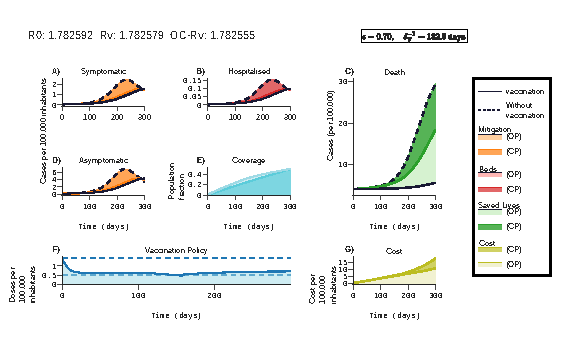
\includegraphics[width=\textwidth]{fig1.pdf}
  \caption{
        Counterfactual scenario regarding no intervention, constant
        vaccination policy (CP), and optimal vaccination policy (OP),
        with vaccination efficiency $\epsilon = 0.7$, induced vaccination
        immunity $\delta_V= 300$ days and vaccination base rate
        $\lambda_V = 50 k/day$.
        Dashed lines denote the prevalence of each class according to
        dynamics with no intervention. Solid lines represent
        the prevalence according to controlled dynamics with the
        optimal or constant vaccination policies. Thus, shaded areas
        respectively denote the gain in
        A) Mitigation of reported symptomatic and B) asymptomatic cases.
        C) Saved lives. D)Coverage, E) Optimal Vaccination policy.
        F)Cost
}
        \label{fig:bocop_scene}
\end{figure}


In \Cref{fig:bocop_scene}, we show a scenario where $\mathcal{R}_0>1$. Despite $\mathcal{R}_v$ remains below but close to $\mathcal{R}_0$.
However, vaccination policies improve the estimated damage.

Vaccination reproductive number $\mathcal{R}_v$, suggests constant policies
according to the mitigation factor
$$
    \left(
        1 -
        \frac{\epsilon \lambda_V}{\mu+\delta_V+\lambda_V}
    \right).
$$
Then disease mitigation is strongly related to vaccine efficiency
$\epsilon$ and vaccination rate $\lambda_v$. Further, given a dynamic with
not vaccine intervention and $\mathcal{R}_0>1$, $\mathcal{R}_v$ suggests a minimal vaccination rate to drive this dynamic to the disease-free state.
In particular, this vaccine efficiency would govern the viability of the
constant policy.



